\chapter{Supplementary Proofs}
\label{app:proofs}

Some results are stated in a chapter because they explain something there, but nothing later in the book depends on them.
Their proofs are collected here so the chapters can keep moving.
Each section says where the result is stated and confirms that no later argument uses it.

\section{Pinsker's inequality}
\label{sec:proof-pinsker}

\Cref{thm:pinsker} in \cref{ch:distances} states that for any distributions $\Pr$ and $\Qr$ on the same sample space,
\[
\TV(\Pr, \Qr) \leq \sqrt{\tfrac12 \KL(\Pr, \Qr)}.
\]
It is there to say that a fit that is good in KL is good for every probability computed from it.
\textbf{Nothing later in the book depends on it}: no theorem, proof or exercise after \cref{ch:distances} uses Pinsker's inequality, and you can skip this section without losing anything.

\optionalproof{Two steps. First prove the inequality for two Bernoulli distributions, by calculus in one variable. Then show that collapsing $\Pr$ and $\Qr$ to `in the event $A^\star$ or not' turns them into two Bernoullis with the same total variation and no larger KL divergence. The second step uses the same tangent-line bound $-\log y \geq 1 - y$ as the proof that KL is nonnegative (\cref{prop:kl-properties}).}

\subsection*{Step 1: two Bernoulli distributions}

\begin{lemma}
\label{lem:pinsker-bern}
For $p, q \in (0, 1)$,
\[
\KL(\Bern(p), \Bern(q)) = p \log\frac{p}{q} + (1 - p)\log\frac{1 - p}{1 - q} \geq 2(p - q)^2.
\]
The inequality also holds for $p \in [0, 1]$ and $q \in (0, 1)$, with the convention $0 \log 0 = 0$.
\end{lemma}

\optionalproof{Fix $p$, treat the gap between the two sides as a function of $q$, and show by its derivative that it is smallest, and equal to $0$, at $q = p$.}
\begin{proof}
Fix $p$ and look at the gap as a function of $q$:
\[
g(q) = p \log\frac{p}{q} + (1 - p)\log\frac{1 - p}{1 - q} - 2(p - q)^2.
\]
At $q = p$ both terms are $0$, so $g(p) = 0$.
Differentiate in $q$:
\[
g'(q) = -\frac{p}{q} + \frac{1 - p}{1 - q} + 4(p - q).
\]
The first two terms combine over the common denominator $q(1 - q)$: $-p(1 - q) + (1 - p)q = q - p$. So
\[
g'(q) = \frac{q - p}{q(1 - q)} - 4(q - p) = (q - p)\left( \frac{1}{q(1 - q)} - 4 \right).
\]
The product $q(1 - q)$ is at most $\frac14$, since $\frac14 - q(1 - q) = (q - \frac12)^2 \geq 0$ (it is the variance of one Bernoulli observation, largest for a fair coin).
So $1/(q(1 - q)) \geq 4$ and the bracket is never negative.
The sign of $g'(q)$ is therefore the sign of $q - p$: $g$ decreases until $q = p$ and increases after.
Its smallest value is $g(p) = 0$, so $g(q) \geq 0$ for every $q$.
\end{proof}

\Cref{fig:pinsker} draws the lemma.
The divergence curve sits above the parabola $2(p - q)^2$ and touches it only at $q = p$.
Near $q = p$ the two are close: the divergence is approximately $(p - q)^2/(2p(1 - p))$ (\cref{sec:dist-kl}), and $1/(2p(1-p)) \geq 2$, with equality only for $p = \frac12$.
The parabola $2(p-q)^2$ is the divergence's own parabola for the hardest case, the fair coin, and every other Bernoulli curves up faster.

\begin{figure}[htbp]
\centering
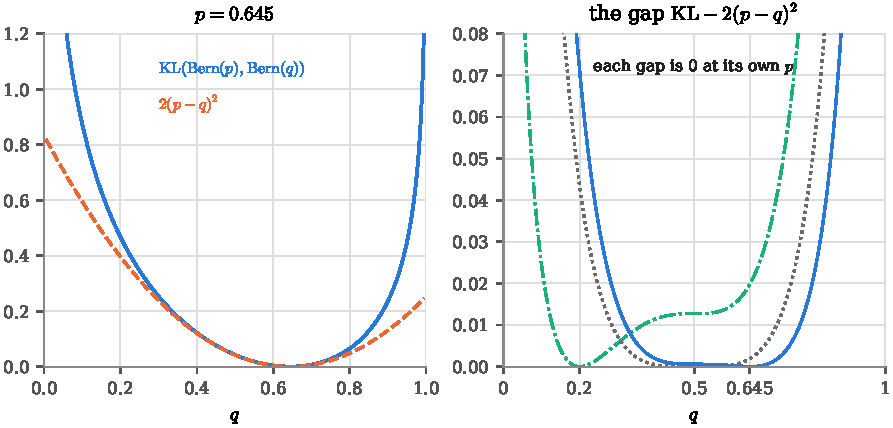
\includegraphics[width=\textwidth]{fig_pinsker}
\caption{The Bernoulli case of Pinsker's inequality. Left: with $p = 0.645$, $\KL(\Bern(p), \Bern(q))$ (blue) lies above $2(p - q)^2$ (orange, dashed) and touches it only at $q = p$. Right: the gap between the two for $p = 0.2$ (aqua, dash-dot), $0.5$ (gray, dotted) and $0.645$ (blue, solid); each gap is $0$ at $q = p$ and positive elsewhere.}
\label{fig:pinsker}
\end{figure}

For the kiss data, $p = 80/124$ and $q = \frac12$: $\KL = 0.0428$ and $2(p - q)^2 = 2 \times 0.1452^2 = 0.0422$.
Taking square roots, $\abs{p - q} = 0.1452 \leq \sqrt{0.0428/2} = 0.1462$.
Since $\TV(\Bern(p), \Bern(q)) = \abs{p - q}$, the lemma is Pinsker's inequality for Bernoulli distributions.

\subsection*{Step 2: reducing any pair of distributions to two Bernoullis}

\begin{lemma}[The log-sum inequality]
\label{lem:log-sum}
For nonnegative numbers $a_1, \ldots, a_k$ and nonnegative numbers $b_1, \ldots, b_k$ with $b_i > 0$ whenever $a_i > 0$, and with $a = \sum_i a_i > 0$ and $b = \sum_i b_i$,
\[
\sum_{i=1}^k a_i \log\frac{a_i}{b_i} \geq a \log\frac{a}{b},
\]
with the convention $0 \log 0 = 0$.
The same holds with the sums replaced by integrals over a region.
\end{lemma}

\optionalproof{Rewrite the difference of the two sides as a weighted average of $-\log$ of ratios and apply the tangent-line bound $-\log y \geq 1 - y$ to each.}
\begin{proof}
Only the terms with $a_i > 0$ contribute on the left. For those, write
\[
\sum_{i: a_i > 0} a_i \log\frac{a_i}{b_i} - a\log\frac{a}{b} = \sum_{i: a_i > 0} a_i \log\left( \frac{a_i}{b_i} \cdot \frac{b}{a} \right) = \sum_{i: a_i > 0} a_i \left[ -\log\left( \frac{b_i}{a_i} \cdot \frac{a}{b} \right) \right],
\]
using $\sum_{i: a_i > 0} a_i = a$ to bring $a\log(a/b)$ inside the sum.
Apply $-\log y \geq 1 - y$ to each bracket:
\[
\geq \sum_{i: a_i > 0} a_i \left( 1 - \frac{b_i}{a_i}\cdot\frac{a}{b} \right) = a - \frac{a}{b}\sum_{i: a_i > 0} b_i \geq a - \frac{a}{b} \cdot b = 0.
\]
The last step uses that the $b_i$ with $a_i > 0$ add up to at most $b$.
For integrals the same lines go through with $\int$ in place of $\sum$.
\end{proof}

In words: lumping several outcomes into one can only lower the divergence.
If you record only whether an outcome fell in a set, and not which outcome it was, the evidence it carries cannot go up.

\optionalproof{Collapse both distributions to the indicator of $A^\star$: total variation is unchanged, KL can only fall (\cref{lem:log-sum}), and for the two resulting Bernoullis \cref{lem:pinsker-bern} applies.}
\begin{proof}[Proof of \cref{thm:pinsker}]
If $\KL(\Pr, \Qr) = +\infty$ there is nothing to prove, so assume it is finite; then $q(x) > 0$ wherever $p(x) > 0$.
Let $A^\star = \{x : p(x) > q(x)\}$, and write $a = \Pr(A^\star)$, $b = \Qr(A^\star)$.
By \cref{prop:tv-area}, $\TV(\Pr, \Qr) = a - b$. If $a = b$, $\TV = 0$ and there is nothing to prove, so assume $a > b$; then $0 < a$ and $b < 1$.

Split the sum (or integral) defining $\KL(\Pr, \Qr)$ into the part over $A^\star$ and the part over its complement, and apply \cref{lem:log-sum} to each part, with $a_i = p(x)$ and $b_i = q(x)$:
\[
\KL(\Pr, \Qr) = \sum_{x \in A^\star} p(x)\log\frac{p(x)}{q(x)} + \sum_{x \notin A^\star} p(x)\log\frac{p(x)}{q(x)} \geq a\log\frac{a}{b} + (1 - a)\log\frac{1 - a}{1 - b}.
\]
(If a part has total $\Pr$-probability $0$, it contributes $0$ on both sides.)
The right-hand side is $\KL(\Bern(a), \Bern(b))$, the divergence between the two distributions of the indicator $\ind\{X \in A^\star\}$.
By \cref{lem:pinsker-bern} (in the extended form for $a \in [0, 1]$; if $b = 0$ the divergence on the right is $+\infty$, which contradicts the finite left side, so $b \in (0, 1)$),
\[
\KL(\Pr, \Qr) \geq \KL(\Bern(a), \Bern(b)) \geq 2(a - b)^2 = 2\,\TV(\Pr, \Qr)^2.
\]
Divide by $2$ and take square roots.
\end{proof}

\begin{intuition}[why the proof works]
Total variation is decided by one event, $A^\star$, where $\Pr$ beats $\Qr$.
Throw away everything about an outcome except whether it fell in $A^\star$.
That leaves a coin, with probability $a$ under $\Pr$ and $b$ under $\Qr$, and the same total variation $a - b$.
Lumping can only lower KL, so the coin's KL is at most the original one.
And for coins, the lemma says KL is at least twice the squared total variation.
\end{intuition}

\section{Each step of the EM algorithm raises the likelihood}
\label{sec:proof-em}

\Cref{sec:lik-em} in \cref{ch:likelihood} states that one E step followed by one M step never lowers the log-likelihood of a mixture.
It explains the climbing curves of \cref{fig:emfaithful}.
\textbf{Nothing later in the book depends on it.}

\optionalproof{Split the log-likelihood of the observed data into two pieces: the quantity the M step maximizes, minus a term that measures how well the parameter predicts the hidden labels. The M step raises the first piece. The second piece can only fall away from its value at the current parameter, by an amount that is a KL divergence and so is never negative.}

\begin{proof}
Write $\theta$ for all five parameters, $\theta_t$ for the current values and $\theta_{t+1}$ for the values after one E step and one M step.
For observation $i$, with hidden label $z \in \{0, 1\}$, let $p_\theta(x_i, z)$ be the joint probability (density in $x_i$) of the observation and the label, $p_\theta(x_i) = \sum_z p_\theta(x_i, z)$ the mixture density, and $p_\theta(z \mid x_i) = p_\theta(x_i, z)/p_\theta(x_i)$ the conditional probability of the label.
Write $q_i(z) = p_{\theta_t}(z \mid x_i)$ for the current weights: $q_i(1) = w_i$ and $q_i(0) = 1 - w_i$.

For any $\theta$ and each $z$, $\log p_\theta(x_i) = \log p_\theta(x_i, z) - \log p_\theta(z \mid x_i)$. Average this over $z$ with the weights $q_i(z)$, which add up to $1$, and add over $i$:
\[
\ell_n(\theta) = \underbrace{\sum_{i=1}^n\sum_z q_i(z)\log p_\theta(x_i, z)}_{Q(\theta)} \; - \; \underbrace{\sum_{i=1}^n\sum_z q_i(z)\log p_\theta(z \mid x_i)}_{H(\theta)}.
\]
$Q(\theta)$ is the complete-data log-likelihood with each label replaced by its weight, which is exactly what the M step maximizes over all five parameters (\cref{ex:lik-em-mstep}), so $Q(\theta_{t+1}) \geq Q(\theta_t)$.
This holds for the sum over $i$, not observation by observation: a step can lower the density of some observations while raising the total.
For the second term,
\[
H(\theta_t) - H(\theta) = \sum_{i=1}^n \sum_z q_i(z)\log\frac{p_{\theta_t}(z \mid x_i)}{p_\theta(z \mid x_i)} = \sum_{i=1}^n \KL\big(p_{\theta_t}(\cdot \mid x_i),\, p_\theta(\cdot \mid x_i)\big) \geq 0
\]
by \cref{prop:kl-properties}, term by term, since $q_i = p_{\theta_t}(\cdot \mid x_i)$.
So $H(\theta_{t+1}) \leq H(\theta_t)$, and
\[
\ell_n(\theta_{t+1}) - \ell_n(\theta_t) = \big(Q(\theta_{t+1}) - Q(\theta_t)\big) + \big(H(\theta_t) - H(\theta_{t+1})\big) \geq 0.
\]
\end{proof}

Ascent says nothing about where the climb ends: EM stops where the gradient of $\ell_n$ is $0$, which can be a local maximum or a saddle point.
